\section{Скриншоты}

\subsection{Главное меню}
\begin{figure}[H]
  \centering
  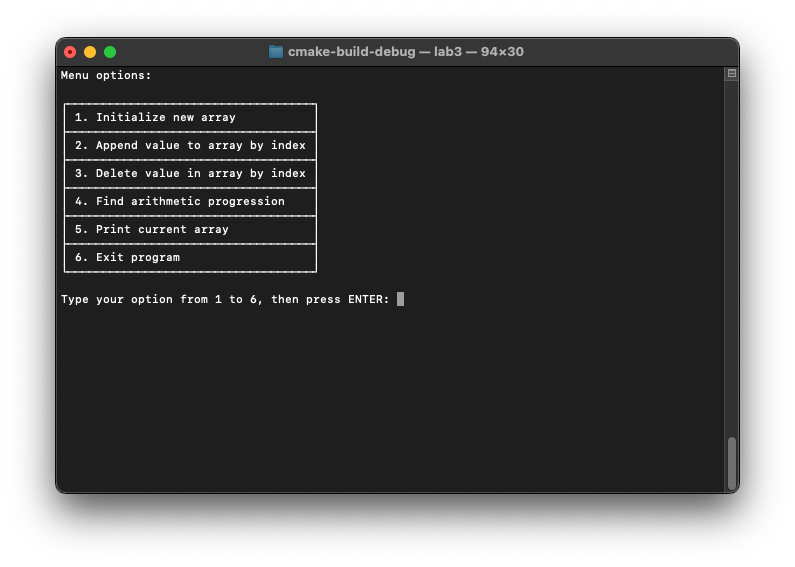
\includegraphics[width=0.75\textwidth]{screenshot_menu}
  \caption{Главного меню и ожидание выбора.}
\end{figure}

\subsection{Создание массива}
\begin{figure}[H]
  \centering
  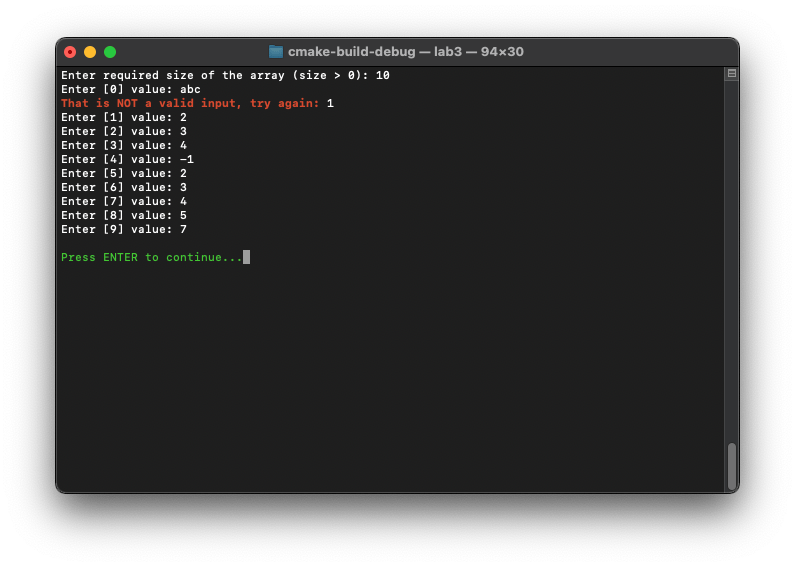
\includegraphics[width=0.75\textwidth]{screenshot_create}
  \caption{Создание массива длинной в 10 элементов.}
\end{figure}

\subsection{Добавление элементов}
\begin{figure}[H]
  \centering
  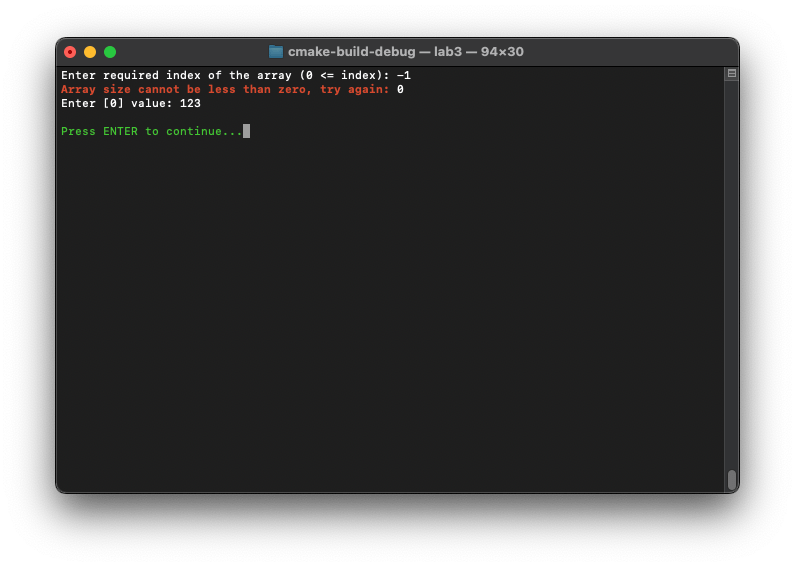
\includegraphics[width=0.75\textwidth]{screenshot_append}
  \caption{Добавление элемента 123 по индексу 0.}
\end{figure}

\subsection{Удаление элементов}
\begin{figure}[H]
  \centering
  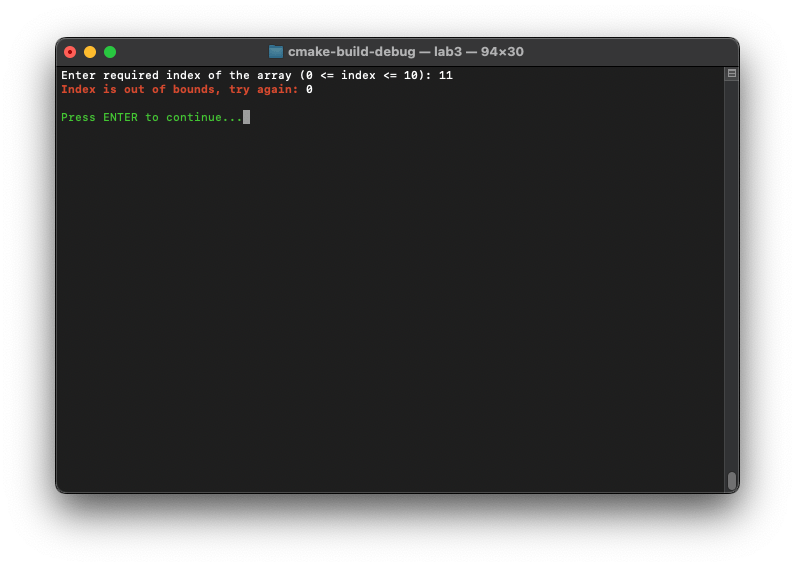
\includegraphics[width=0.75\textwidth]{screenshot_remove}
  \caption{Удаление элемента по индексу 0.}
\end{figure}

\subsection{Поиск арифметической прогрессии в цифрах элементов}
\begin{figure}[H]
  \centering
  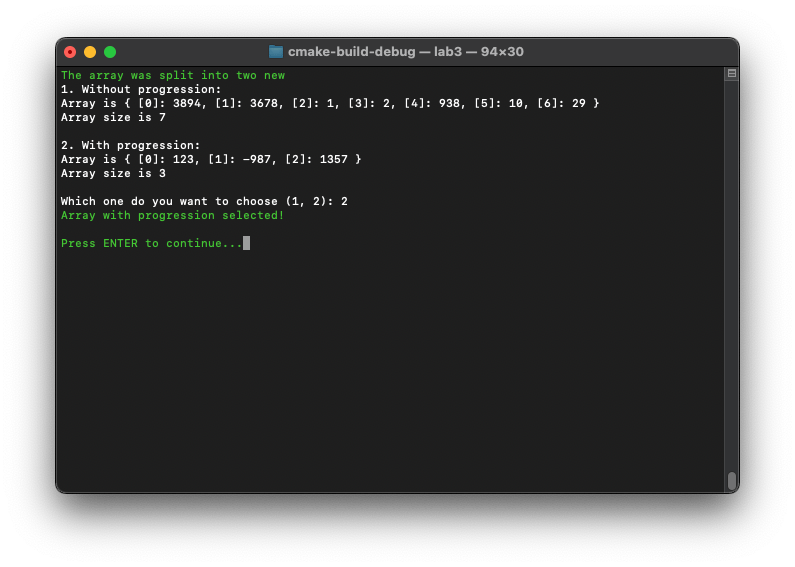
\includegraphics[width=0.75\textwidth]{screenshot_progression}
  \caption{Получение массива с арифметической прогресии в цифрах элементов.}
\end{figure}

\subsection{Вывод массива}
\begin{figure}[H]
  \centering
  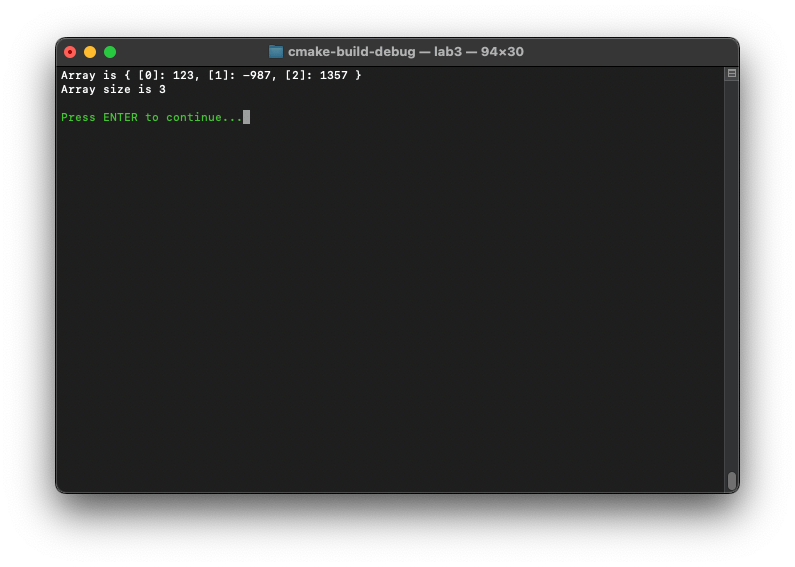
\includegraphics[width=0.75\textwidth]{screenshot_print}
  \caption{Вывод всех жлементов массива и его длины.}
\end{figure}

\subsection{Использование памяти}
\begin{figure}[H]
  \centering
  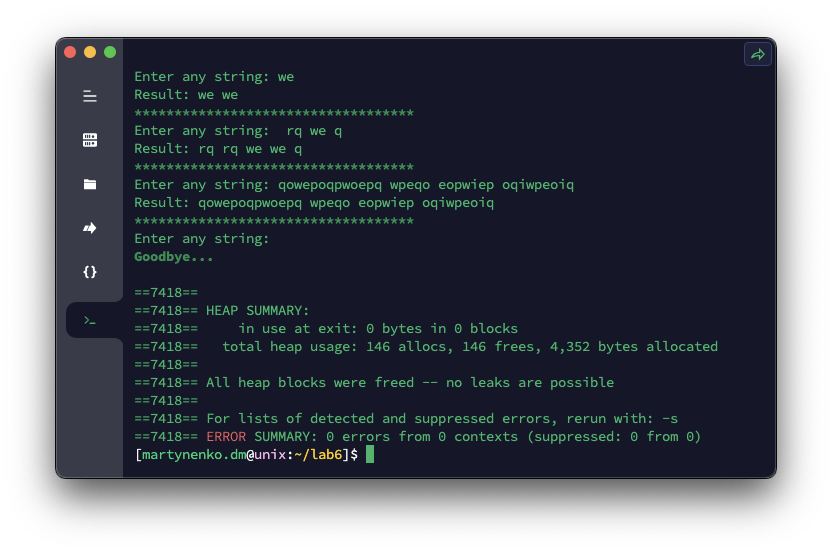
\includegraphics[width=0.75\textwidth]{screenshot_valgrind}
  \caption{Успешная проверка использования памяти при помощи valgrind.}
\end{figure}
